\chapter{Problem Statement and Requirements}

%With all of the focus on self-driving vehicles we have chosen to specifically take a closer look at how buses can be automated to fulfil their objectives as if driven by a person. 

%\section{Problem}
%-\todo{Fix title}.\\
%\unsure{isn't the introduction the problem?}
%\section{Problem Statement}

\textbf{Is it possible to create a self-driving bus using LEGO hardware, that is able to perform the functionality required of a typical bus, in a scaled down version of the pre-existing infrastructure.}
\info{In this version of the problem statement it is already specified from the very start that the focus is on the LEGO.}
%\textbf{Is it possible to create a self-driving bus while working within the hardware limitations of LEGO, that is able to perform the functionality required of a typical bus, in a scaled down version of pre-existing infrastructure.}

\section{Brainstorm}

A brainstorm was made in order to find the potential functionality an autonomous bus could implement in the context of the problem statement. The results of the brainstorm and a short description of each feature is shown below. 

\begin{description}
\item [Follow Track]
The general idea here is to drive within a set of boundaries, like road markings.

\item[Stop Button]
A way to signal the bus that some passengers want to get off at the next bus stop.\unsure{source needed?}

\item[Detect Bus Stop]
Detection of a marker or a sign that indicates where the bus stop is located.

\item[Switch Lanes]
This functionality allows the bus to switch into and out of the lane in which the bus stop is located, and also allows overtaking other vehicles. 

\item[Overtake]
Allows the bus to overtake a stopped or slow vehicle. 

\item[Speed Limiter]
A limiter that enforces a designated speed, making sure that it speeds up/slows down to match the speed limit.

\item[Cruise Control]
Staying behind a moving object without constantly accelerating and braking, thereby providing a smooth journey.

\item[Detecting Obstacles]
The ability to detect obstacles, such that it can brake or manoeuvre to prevent crashes.

\item[Door]
Controlling one or multiple doors to allow passengers to get on and off the bus.

\item[Intersections]
An intersection is a regular occurrence in the pre-existing infrastructure; it is therefore useful for the bus to be able to navigate them, whilst following traffic regulations.

\item[Roundabouts]
Like intersections, roundabouts are found in pre-existing infrastructures.

\item[Passenger Limit]
As per fire safety rules, only a set amount of passengers are allowed within any certain space at time. To conform to these rules, there should be some system that counts the passengers entering and leaving the bus.

\item[Transformer Bus]
Being able to combine or split buses allows for more flexibility in regards to making sure there's always sufficient space on the buses, which may vary for each route. 

\item[Dark Sensor]
Power can be saved if the bus only turns on the headlights when they are needed.\info{Isn't it illegal to have the lights turned off?}

\end{description}

%\unsure{A brainstorm was made based on our problem statement, to find all the potential useful functionality}













\section{Prioritising Brainstorm Ideas}

Due to the inherent limitations of the project, some functionality has to be excluded. To help determine which functionality should be the focus points, an evaluation was made according to the Risk Vs Value model to help prioritise the ideas. 

The Risk Vs Value model works by having the individual members of the development team evaluate each different functionality individually and giving them a risk and a value. Each of the values and risks is represented by a number from 0 to 100, where 100 value means that the functionality on its own will complete the project, and 0 provides nothing to the project. A 100 risk is something that will take all our time, and 0 is done without committing any time. 

In this project, each of the members of the development team wrote their evacuation without talking to each other or knowing the evaluation of the other members. Afterwards, the team revealed their numbers and the highest and the lowest would each explain why they evaluated it the way they did. After the explanation, the members of the group had the opportunity to change their evaluation. Using this approach produced the graph \ref{fig:RiskValueGraph}.

\begin{figure}[!h]
    \centering
	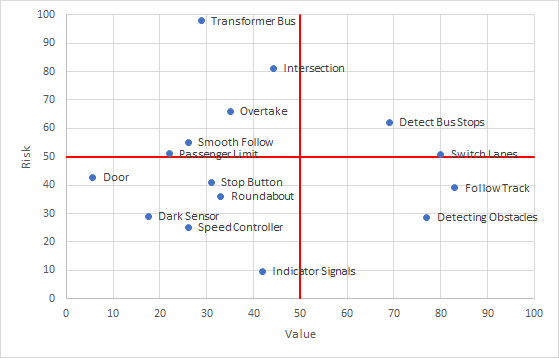
\includegraphics[width=0.9\textwidth]{Images/Graphs/RiskValue.png}
    \caption{Risk Value Graph}
    \label{fig:RiskValueGraph}
\end{figure}

According to the Risk Vs Value model, the development should start with the tasks with a high risk and value, then proceed with the tasks with low risk and high value, and lastly the tasks with low value and low risk. Where the tasks with high risk and low value should not be focused at all. 

According to the model, we should start detecting bus stops, and then prioritise the functionality according to a clockwise rotation. However there will never be any model that works as a silver bullet, and the relations and dependencies between the different functionality must be taken into account.  

\subsection{Priority Modifications}

In this section, we will give lower or higher priorities to some features, dependant on the relations between the different features.

All of the passenger functionality is completely reliant on the driving functionality. Because of this, everything concerning passengers was given low priority. The same reasoning is given to roundabouts, overtakes and intersections because these are also reliant on functional driving. Dark sensor is also given lower priority based on its low value.

Follow track is essential, which is why it has the highest value, to almost everything else, and has therefore been given higher priority.




\section{Project Requirements} \todo{Should be made more specific} \label{Requirements}
In this section we describe the requirements that the final product will need to meet in order to solve the problem statement. %...the requirements for the project will be described. The requirements are meant to be guidelines for the project and the goals which need to be met. The order of appearance is dependant on their importance.

%To test if the bus is able to meet its requirements, test tracks will be constructed. The requirements for the track and the bus will be specified below.
\info{This section should concern additional elaboration of the chosen requirements from the brainstorm. It should not contain design choices, and it is also doubtful that the requirements should be split into vehicle requirements and track requirements.}

%\subsection{Vehicle Requirements}
%Metatext

\begin{description}
    \item [(1) Follow Track]
    The bus needs to be able to detect the lines marking the edges of a road lane and stay within these. The relation between the size of the track and the LEGO bus should be the same as the relation real busses have with real roads. This also applies to the turning degrees of real road turns. 
    
    \item[(2) Stop at Bus Stops]
    The bus needs to detect and stop at bus stops on its route and resume driving afterwards. 

    \item[(3) Switching Lanes] 
    The vehicle should be able to switch lanes, useful both for overtaking other vehicles and stopping at a bus stop in a dedicated lane. 
    
    \item[(4) Detecting Obstacles]
    Detecting obstacles is a crucial part of preventing crashes and other potential accidents. As such the bus needs to be able to detect obstacles in front of it and perform preventative measures to prevent the collision. Implemented in the real world, the response, response time and field of view should be at least on par with normal human drivers. Seeing as this is highly improbable and unnecessary for a LEGO bus, we will consider this requirement fulfilled as long as it can: detect and react to obstacles in a 60 degree cone to the front within less than a second, and detect and react to obstacles within a 150 degree arch whenever the vehicle is switching lanes. \unsure{what are the rules for human? How many degrees do they need to watch (counting the mirrors)?}
    
    \item[(5) Stop Button]
    Busses, unlike trains, are not required to stop at every bus stop, and as such need a button that allows the passengers to signal at which stops they want to get off at. The bus should be able to at any given time receive a signal, and processes this signal as theoretical passengers wanting to get of the bus.
    
    \item[(6) Speed Limiter]
    The bus should have a speed limiter which can detect the current speed limits and keep the specific velocity in the different speed zones. It should be able to switch between at least 2 different speeds, given 2 different signals/physical signals.
    
    \item[(7) Indicator Signals]
    Signalling that a vehicle wants to turn is very helpful for the other vehicles on the road. The bus should have some way of indicating to the surroundings that it is turning/going to turn.
\end{description}

%\subsection{Lego vehicle and sensors requirements}
%This subsection will decide upon the requirements for the LEGO bus and the sensors that it uses.

%\subsubsection{Motors}
%The LEGO vehicle should use two servo motors\unsure{is this not a design thing? why is this a requirement}? One for the turning mechanism and one for driving forward and backwards. The turning mechanism should be the front wheels. 
%The LEGO bus needs a number of motors in other to drive itself forwards and backwards and in order to steer.\info{Have changed this subsection to be much less specific.}






% table overview with rankings of both track and car + prototypes